%==============================================================================
\chapter{Detector}
\label{sec:det}
%==============================================================================

In this chapter, a detailed description of the proposed PINGU neutrino
telescope and its predecessor IceCube will be given. We will start with
introducing the concept of ice or water based neutrino telescopes based on the
detection of Cherenkov radiation with IceCube/DeepCore as example, followed by
a characterisation of its upcoming PINGU upgrade.
Thereafter we will discuss how physics events will be selected and
reconstructed in an analysis targeting the determination of the neutrino mass
hierarchy, and finally how conceptually new hardware might improve the results.

%==============================================================================
\section{IceCube/DeepCore}
\label{sec:ICDC}
%==============================================================================

\subsection{Location}
\label{sec:IClocation}

As already mentioned (Sec.~\ref{sec:NuDetection}), the natural choice for
observing the low natural fluxes of high energy neutrinos are water-based
Cherenkov detectors. Although the basic requirement---a sufficiently large
amount of water or ice---seems not very difficult to meet, there are additional
constraints that have to be addressed as well:

\begin{description}
 \item[Size:] Depending on the energy range one is interested in, the size of
  the detector has to be adjusted accordingly. Since the atmospheric flux
  decreases rapidly with increasing energy, one needs larger detectors to study
  higher fluxes. Roughly from the GeV scale upwards, the required dimensions are
  so big (several hundred metres) that artificial structures like the
  underground caverns of Kamiokande and Super-Kamiokande \cite{SuperKosc} are
  not feasible any more and one has to look for suitable natural locations.
 \item[Transparency:] Since the detection of neutrinos is based on recording
  Cherenkov radiation, i.\,e.\ photons in the optical and near UV regime,
  obviously the chosen medium has to be transparent for these photons. Here ice
  has an advantage over fluid water as it has very low absorption down to
  wavelengths of 300\,nm and below \cite{IceProps}, while the fluid starts to
  absorb significantly below 400\,nm \cite{WaterAbs}.
 \item[Purity:] Usually the experiments try to reconstruct the neutrino events
  as accurately as possible. Therefore it is desirable to record a large number
  of unscattered photons and hence a very clear environment\footnote{There might
  be, however, situations where scattering is desired, e.\,g.\ when only the
  neutrino energy is of interest, then strong scattering keeps the photons
  inside the detector for a longer time and hence increases the total number
  of detected photons, thereby improving the energy resolution}.
 \item[Shielding:] In high energy neutrino experiments, muons from atmospheric
  showers created by cosmic radiation (cf.\ Sec.~\ref{sec:AtmNus}) are a
  background process whose rate is several orders of magnitude higher than the
  neutrino signal. In order to suppress those muons, detectors have to be
  placed deep underground so that there is a shielding with several hundred
  meters thickness, comparable to the range of $\mathcal{O}
  (100\,\mathrm{GeV})$ muons.
\end{description}

\begin{figure}[htp]
 \centering
 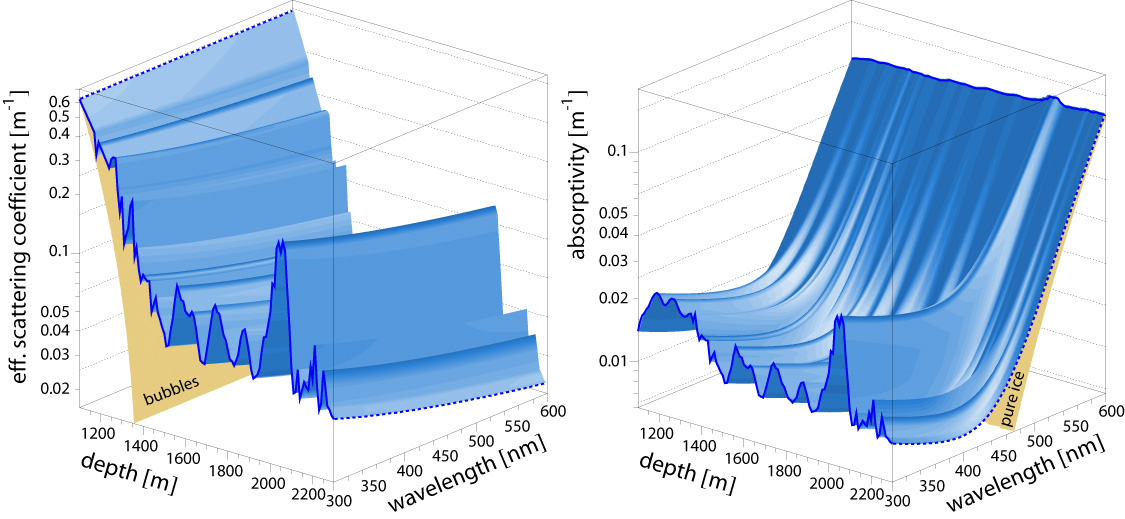
\includegraphics[width=\textwidth]{Icepaper_figure22_scatt-abs-length}
 \caption{Effective scattering and absorption of light in the polar ice. Plot 
  taken from \cite{IceProps}.}
 \label{fig:ice_scatt_abs}
\end{figure}

Choosing an environment optimising all these factors, the IceCube neutrino 
observatory has been constructed in the deep glacial ice at the geographical 
South Pole in Antarctica. The Antarctic glacier with its thickness of $\approx 
2500$\,m is a pristine environment of substantial size. In contrast to natural 
resources like lakes or the deep sea, it inherently provides a solid holding 
structure for the instrumentation, is free of lifeforms that might disturb or 
even destroy the detector, and has a much lower content of radioactive $^{40}$K 
than sea water. Especially at depths more than $\approx 2000$\,m below the 
surface, age and high pressure have facilitated the hydratisation of enclosed 
air bubbles, leaving an extremely clear ice with scattering and absorption 
lengths of several tens of metres even in the UV range, see 
Fig.~\ref{fig:ice_scatt_abs}. Instrumenting only the deepest ice below 1500\,m 
guarantees a sufficient shielding of atmospheric muons. 

The nearby Amundsen-Scott South Pole Station operated by the United States 
Antarctic Program provides the infrastructure needed for such a large scale 
experiment. This incorporates the supply of electrical power for the detector 
itself and the computing farm processing the raw data, satellite communications 
for transmitting science data, general technical support as well as 
accommodations for the visiting scientists.

\subsection{Detector Geometry}
\label{sec:ICgeometry}

A total of 86 strings, each instrumented with 60 Digital Optical Modules (DOMs, 
see Sec.~\ref{sec:ICDOM}), have been installed during IceCube's deployment phase 
from 2005 until December 18, 2010. A hot water drill was used to melt holes of 
60\,cm diameter into the ice, reaching down to 2450\,m, shortly above the 
underlying bedrock. Then the strings were lowered into the holes still filled 
with water which then refroze and firmly encloses the strings.

Eighty of those strings form the hexagonal main array with an inter-string 
distance of 125\,m, while the remaining six are placed at additional positions 
near the centre of the array, forming a dense sub-array with a string spacing 
of only 72\,m, lowering the threshold energy for neutrino detection from 
$\approx 100$\,GeV to $\approx 20$\,GeV. A top view of the string layout is 
shown in Fig.~\ref{fig:string_layout}.

\begin{figure}[htp]
 \centering
 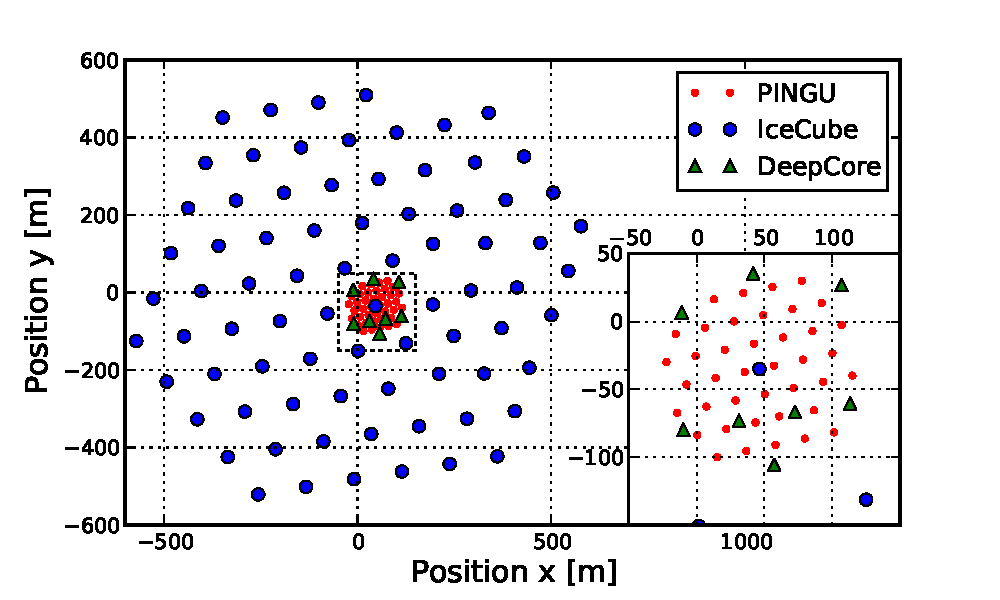
\includegraphics[width=\textwidth]{ic_dc_pingu_strings}
%  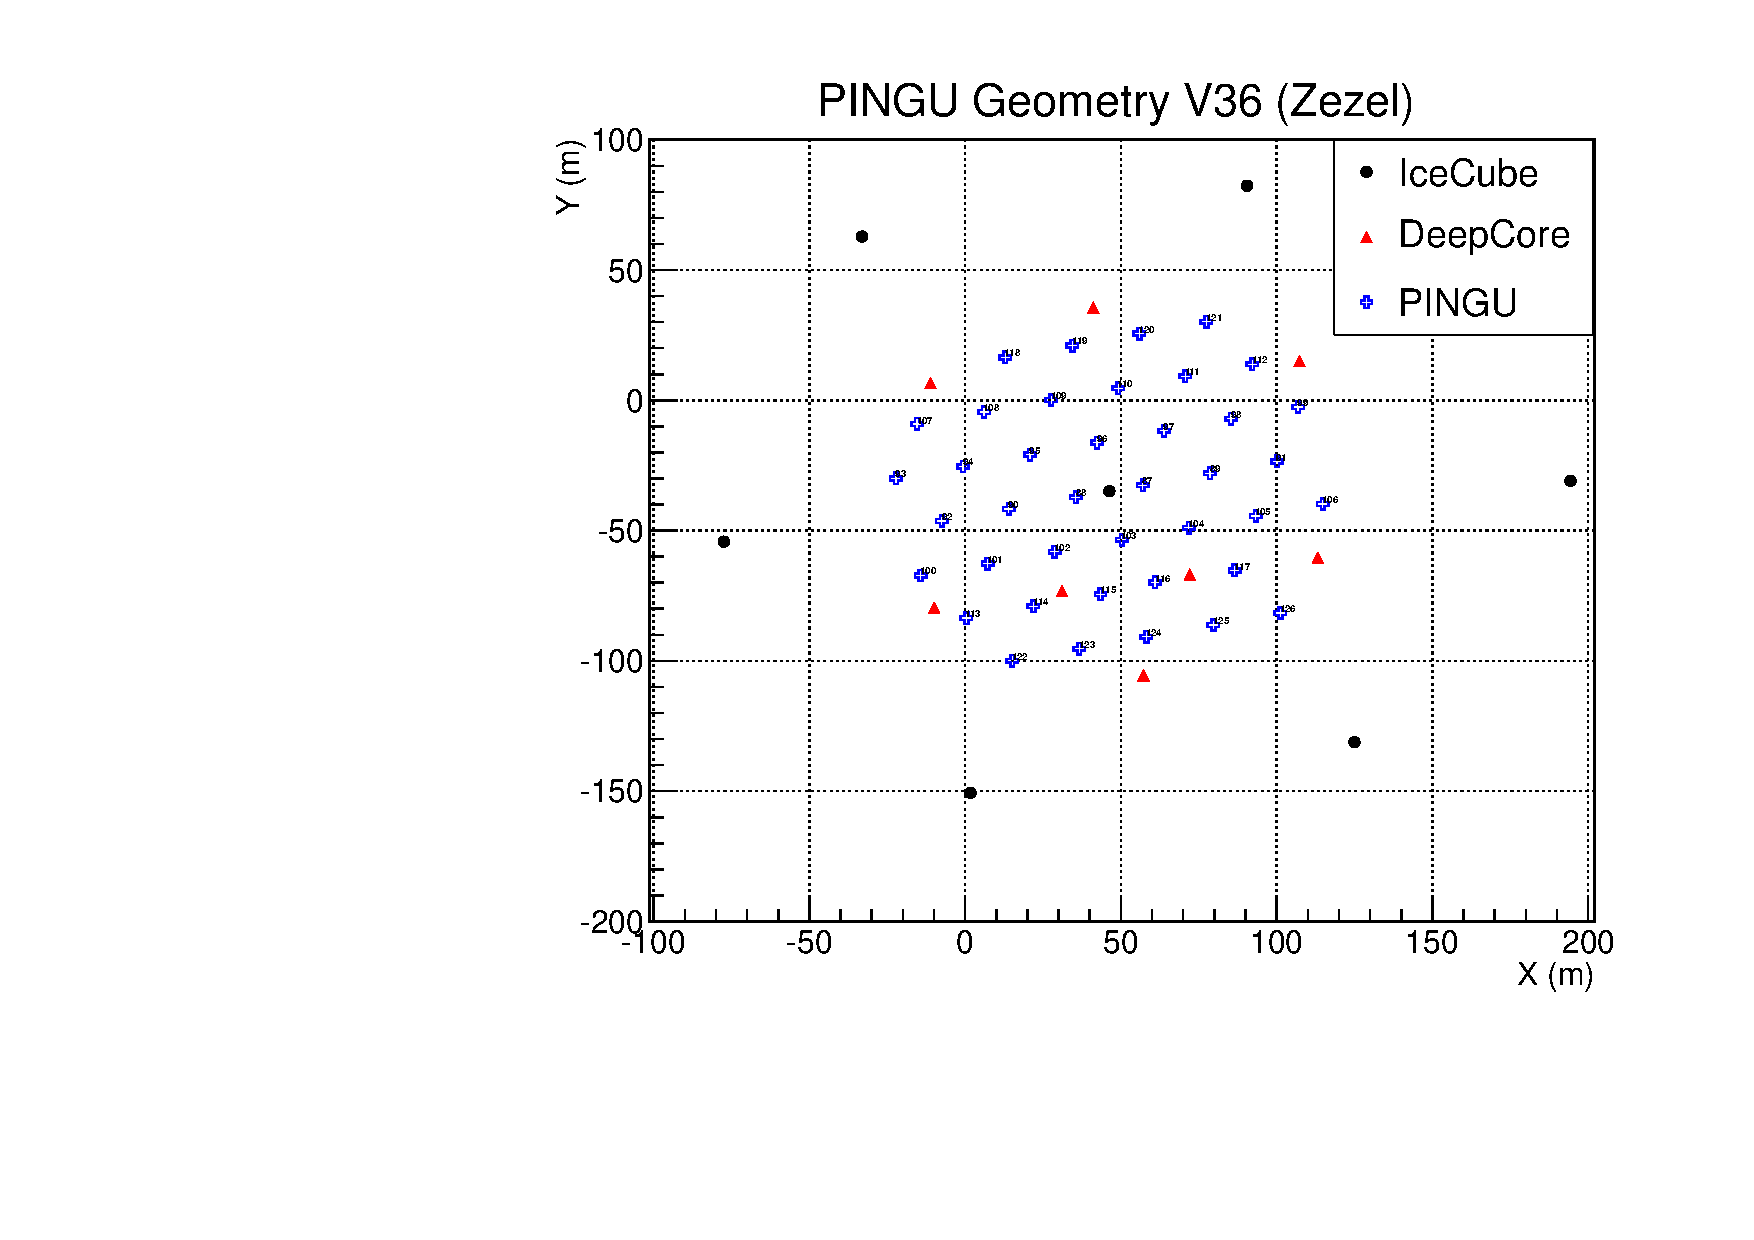
\includegraphics[width=0.7\textwidth]{pingu_V36_Zezel_40_s22_d3}
 \caption{Top view of the IceCube string layout, including the DeepCore and 
planned PINGU (geometry V36) sub-arrays.}
 \label{fig:string_layout}
\end{figure}

To the lowest 1000\,m of the main array strings, sixty DOMs each are attached, 
evenly spaced with a distance of 17\,m. In DeepCore, the vertical DOM spacing 
is only 7\,m below the dust layer found between 1950\,m and 2100\,m 
depth\footnote{The dust layer can be recognised easily in 
Fig.~\ref{fig:ice_scatt_abs} as the region of increased scattering and 
absorption.}, with a veto cap of ten DOMs with 10\,m spacing per DeepCore 
string above it \cite{I3Design,DCDesign}.


\subsection{Digital Optical Modules}
\label{sec:ICDOM}

\begin{figure}[htp]
 \centering
 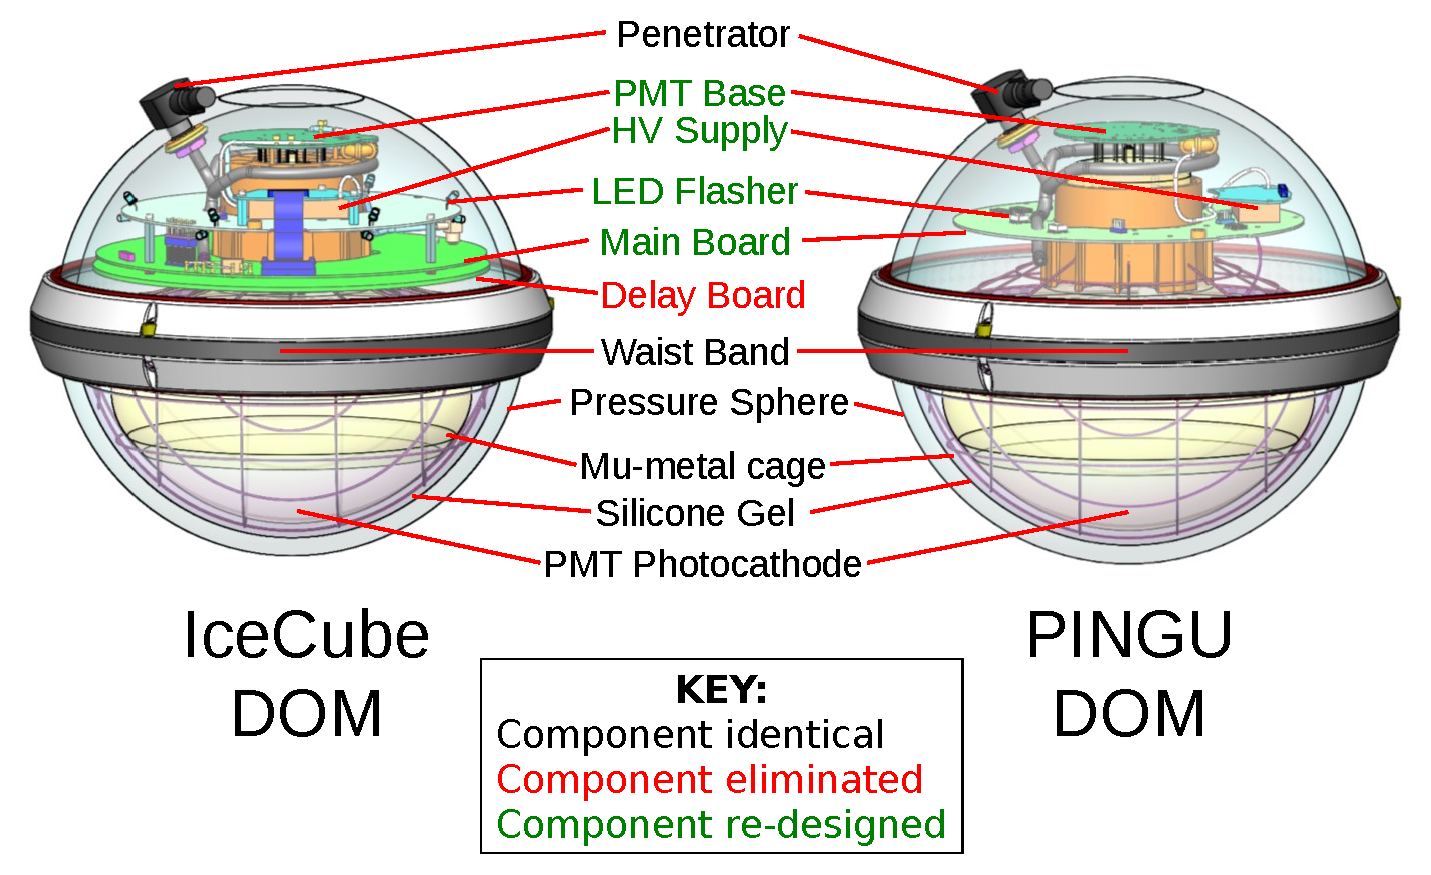
\includegraphics[width=0.7\textwidth]{I3DOM_PDOM_cropped}
 \caption{Comparing an IceCube/DeepCore DOM to the PDOM used in PINGU. Graphics 
taken from \cite{PDOM_Aachen}.}
 \label{fig:DOM}
\end{figure}

The 5160 Digital Optical Modules are the basic detection units of IceCube. They 
are attached to the string and connected to the main string cable during 
deployment and work autonomously except for the low voltage power supply. This 
modular design has the convenience that if one DOM fails to work and cannot be 
fixed as it is frozen in the deep ice, the others are not affected.

As shown in Figure \ref{fig:DOM}, the DOM is housed by a borosilicate glass 
sphere of 13\verb+"+ diameter and 0.5\verb+"+ thickness to withstand the 
pressure arising from the refreezing water in the drill holes. This glass sphere 
also contributes to the noise rate of about 540\,Hz per DOM as it contains 
isotopes of the uranium and thorium decay chains. The content of natural 
$^{40}\mathrm{K}$, that undergoes beta decay where the emitted $\beta$ particle
generates Cherenkov light, has been reduced in the glass.

The main component of the DOM is a 10\verb+"+ photomultiplier tube (Hamamatsu 
R7081-02 \cite{PMTpaper,PMTdata}). In DeepCore, an improved version of this PMT 
with a 35\,\% higher quantum efficiency was used \cite{DCDesign}. The PMT is 
oriented downwards as the main focus of IceCube is on extraterrestrial neutrinos 
from the northern hemisphere that have travelled through the Earth and hence 
arrive at the South Pole from below. The coupling to the glass sphere is 
provided by an optical gel which also provides protection and fixation to the 
PMT, while a surrounding Mu-metal grid guarantees the shielding of external 
magnetic fields.

The upper half of the DOM is filled with an high voltage divider that locally 
transforms the 96\,V voltage that is provided by the string main cable into the 
high voltage of 1.3--1.5\,kV that is needed to fuse the PMT, thus making it 
independent from possible voltage fluctuations of the pole station's power 
supply. Around the HV divider, the circular flasher board and DOM mainboard are 
mounted. The flasher board is populated with LEDs that can be used to produce a 
standardised signal for calibration. On the mainboard the electronics are 
located that are needed to read out the PMT signal and digitise the recorded 
data in situ, after which they are sent to the surface.



%==============================================================================
\section{PINGU}
\label{sec:PINGU}
%==============================================================================

PINGU, the Precision IceCube Next Generation Upgrade, is planned as a further 
infill to the IceCube/DeepCore array, lowering the energy threshold to few GeV 
\cite{LoI}. The current baseline geometry, V36, consists of forty additional 
strings with 96 PINGU-DOMs (PDOMs, see below) each. In this layout, shown in
Fig.~\ref{fig:string_layout}, the string spacing is 22\,m while the PDOMs are
located the lowest 300\,m of IceCube with a vertical distance of 3\,m. In this
depth, the same as the main part of DeepCore, the ice has the best optical 
properties.

This detector geometry has been optimised to yield a maximum sensitivity for 
the neutrino mass hierarchy. It will be used for all studies described in 
Chapter~\ref{sec:ana} unless explicitly stated otherwise.

In terms of hardware and software infrastructure, many things can be adopted 
from IceCube, redesigning parts where a potential for improvement or 
simplification has been discovered. Several components of the electronics part
of the module, like the main board, the PMT base, and the high voltage supply,
have been redesigned or replaced by more recent versions. In particular the PMTs
will all be the high quantum efficiency models already installed in DeepCore.
A delay board has become obsolete with the more recent signal digitisers and
will not be part of the PINGU DOMs. Additional components, such as cameras to
monitor the freeze-in process, are in discussion.

Although the bulk of PDOMs are an improved version of the technology that has 
proven to work reliably, prototypes of novel optical modules will be deployed 
with PINGU as well. As those might be the baseline technology of future 
neutrino telescopes, they have to be tested under realistic conditions before 
they can be considered for large-scale use. Two options for these 
next-generation optical modules are described in Sec.~\ref{sec:Gen2DOM}, 
studies showing how they will impact the NMH determination are presented in 
Sec.~\ref{sec:om_effects}.

Another thing to be improved upon in PINGU is the so-called ``hole ice''. In 
IceCube it was observed that the refrozen ice directly around the strings that 
had been molten during deployment contains lots of small air bubbles. These 
inclusions lead to a dramatically reduced scattering length around the DOMs,
significantly deteriorating the quality of event reconstruction that strongly
profits from a large number of direct (i.\,e.\ unscattered) photons being
recorded. In order to reduce the impact of the hole ice, the molten water will
be degassed as a part of the drilling process for PINGU, thus reducing its air
content and hence the number of air bubbles remaining after refreezing.

%==============================================================================
\section{Event Selection}
\label{sec:EvtSel}
%==============================================================================


%==============================================================================
\section{Event Reconstruction}
\label{sec:EvtReco}
% TODO: maybe move this section to the end of the chapter?
%==============================================================================


%==============================================================================
\section{Next-Generation Optical Modules}
\label{sec:Gen2DOM}
%==============================================================================

Currently two different prototypes of optical modules are supposed to be
deployed in PINGU. The first one, called mDOM (Sec.~\ref{sec:mDOM}), is an
adaptation of the Km3NeT optical module \cite{Km3NeTmodule} whose shape has been
changed from spherical to cylindrical in order to fit into the holes drilled for
the PINGU strings. The other one, called WOM (Sec.~\ref{sec:WOM}), is a novel
approach to enhance the photon collection efficiency by using passive
components.

Both types of modules will be described in more detail below. In
Sec.~\ref{sec:om_effects}, the performance of a PINGU detector consisting fully
of these next-generation modules will be investigated.

\subsection{Multi-PMT Optical Module (mDOM)}
\label{sec:mDOM}

% \begin{figure}[htp]
%  \centering
%  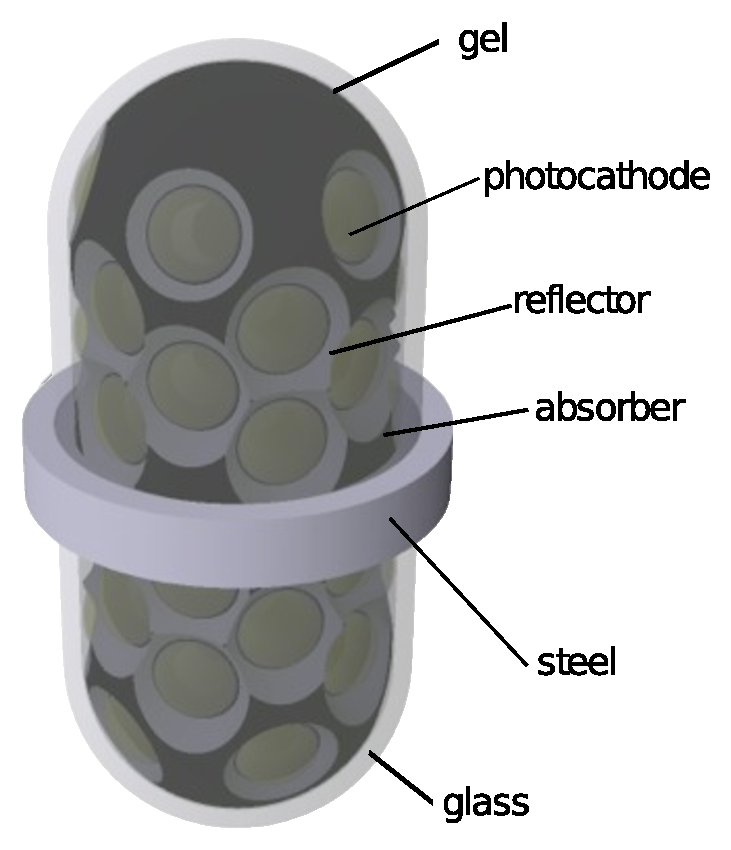
\includegraphics[width=0.5\textwidth]{mDOM_cropped}
%  \caption{The mDOM module concept. Graphics taken from \cite{mDOM_Geneva}.}
%  \label{fig:mDOM}
% \end{figure}

\begin{figure}
\centering
  \subfloat[\label{fig:mDOM}]
    {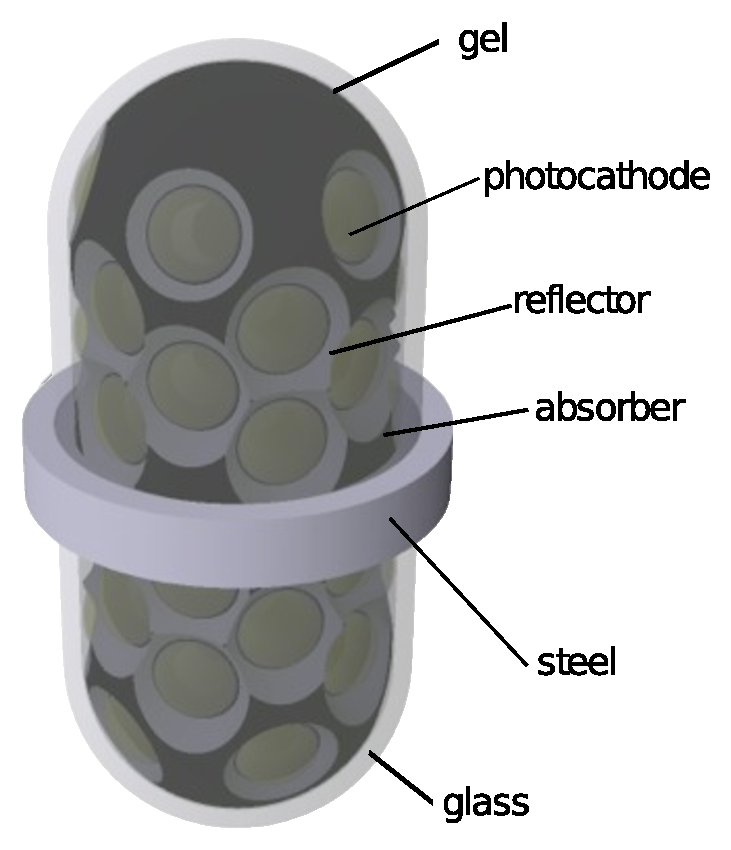
\includegraphics[height=7cm]{mDOM_cropped}}\qquad
  \subfloat[\label{fig:WOM}]
    {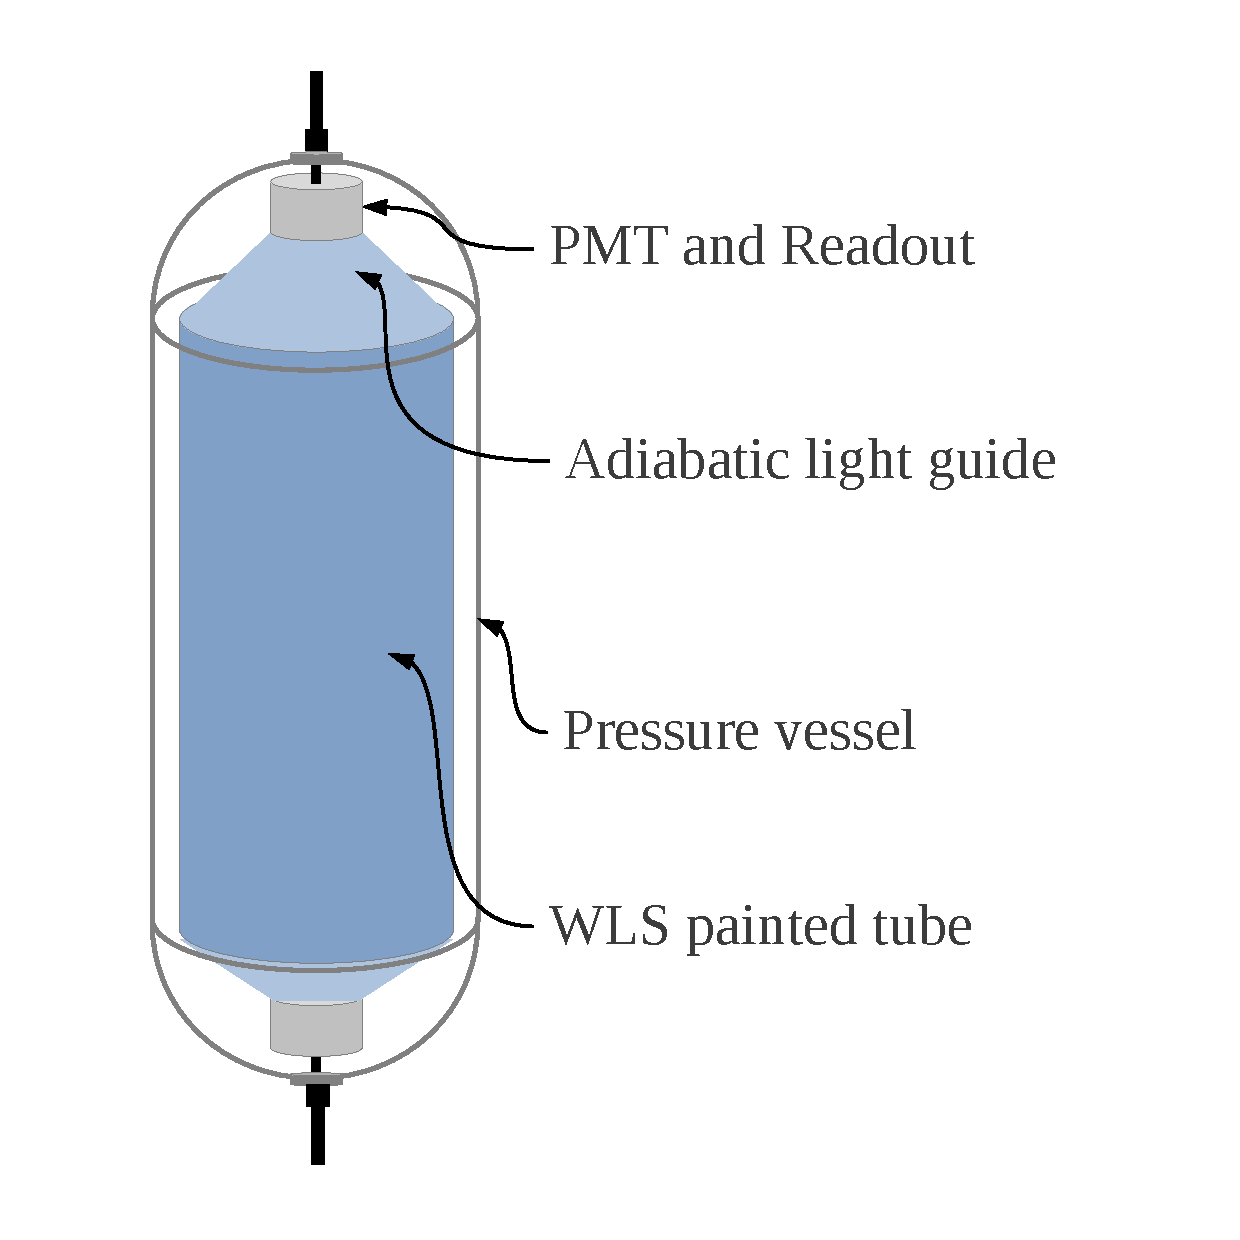
\includegraphics[height=7cm]{WOM}}
  \caption{The \protect\subref{fig:mDOM} mDOM and \protect\subref{fig:WOM} WOM
    module concepts. Graphics taken from \cite{mDOM_Geneva} and \cite{WOM_ICRC},
    respectively.}
\label{fig:Gen3modules}
\end{figure}

Comparing the mDOM, short for Multi-PMT Optical Module, to the standard PINGU
DOMs, the main difference is that instead of one single large PMT, a total of
41 small PMTs with 3\verb+"+ diameter will be used for photon detection, see
Fig.~\ref{fig:mDOM}. The advantages from this layout are that the angular
acceptance covers almost every direction, in contrast to the downwards-pointing
single PMT that has no sensitivity for photons arriving from above.

In addition, the use of more than one PMT per module allows for a very
effective noise reduction. If one only counts module hits where at least two
different PMTs on the same module have registered a photon within a very short
coincidence time, the most important sources of module noise can be strongly
suppressed: Both radioactive decays inside the PMT glass housing and random
electronic noise are restricted to one PMT at a time and hence vetoed with
close to 100\,\% efficiency.

\subsection{Wavelength-shifting Optical Module (WOM)}
\label{sec:WOM}


